%%%%%%%%%%%%%%%%%%%%%%%%%%%%%%%%%%%%%%%%%
% Simple Sectioned Essay Template
% LaTeX Template
%
% This template has been downloaded from:
% http://www.latextemplates.com
%
% Note:
% The \lipsum[#] commands throughout this template generate dummy text
% to fill the template out. These commands should all be removed when 
% writing essay content.
%
%%%%%%%%%%%%%%%%%%%%%%%%%%%%%%%%%%%%%%%%%

%----------------------------------------------------------------------------------------
%	PACKAGES AND OTHER DOCUMENT CONFIGURATIONS
%----------------------------------------------------------------------------------------

\documentclass[12pt]{article} % Default font size is 12pt, it can be changed here

\usepackage{geometry} % Required to change the page size to A4
\geometry{a4paper} % Set the page size to be A4 as opposed to the default US Letter

\usepackage{tabularx}
\usepackage[utf8]{inputenc}


\usepackage{graphicx} % Required for including pictures

\usepackage{float} % Allows putting an [H] in \begin{figure} to specify the exact location of the figure
\usepackage{wrapfig} % Allows in-line images such as the example fish picture

\usepackage{lipsum} % Used for inserting dummy 'Lorem ipsum' text into the template

\usepackage{hyperref}

\usepackage[shortlabels]{enumitem}
                    
\usepackage{xcolor}


\linespread{1.2} % Line spacing

%\setlength\parindent{0pt} % Uncomment to remove all indentation from paragraphs

\graphicspath{{Pictures/}} % Specifies the directory where pictures are stored

\begin{document}
\setlist[enumerate, 1]{1\textsuperscript{o}}

%----------------------------------------------------------------------------------------
%	TITLE PAGE
%----------------------------------------------------------------------------------------

\begin{titlepage}

\newcommand{\HRule}{\rule{\linewidth}{0.5mm}} % Defines a new command for the horizontal lines, change thickness here

\center % Center everything on the page

\textsc{\Large Position Prediction Based on Movement Data}\\[0.5cm] % Major heading such as course name
\textsc{\large System Design Document}\\[0.5cm] % Minor heading such as course title

\vfill

\emph{Authors:}\\
Timo Jockers, Oliver Mänder, Benjamin Moser, \\
Manuel Prinz, Sebastian Strumbelj, Simon Suckut

\vfill % Fill the rest of the page with whitespace

\end{titlepage}

%----------------------------------------------------------------------------------------
%	TABLE OF CONTENTS
%----------------------------------------------------------------------------------------

\tableofcontents % Include a table of contents

\newpage % Begins the essay on a new page instead of on the same page as the table of contents 

%----------------------------------------------------------------------------------------
%	INTRODUCTION
%----------------------------------------------------------------------------------------

% Changelog
\section{Änderungen}


\begin{tabular}{|c|c|p{10cm}|c|}
\hline
Version & Author & Description of changes & Date \\ \hline\hline

%changelog content 
1.0 & SS & \color{red}{Aufbau der App in Android Studio} & x.5.2018 \\\hline
	&	&	&	\\\hline

\end{tabular}


{\small

\noindent
\\\\Legend: \\
SSJ = Sebastian Strumbelj \\
BM = Benjamin Moser \\
MP = Manuel Prinz \\
OM = Oliver Mänder \\
SS = Simon Suckut \\
TJ = Timo Jockers \\
ALL = SSJ, BM, MP, OM, SS, TJ \\
}


%------------------------------------------------

\section{Einleitung} % Major section

%------------------------------------------------

\subsection{Zweck}
Das Erstellen einer App, um einem Ornithologen das Finden eines Vogels zu erleichtern, indem sie dessen zukünftige Position mit einem Vorhersagemodell abschätzt. 

%------------------------------------------------

\subsection{Design-Ziele}

Diese Dokumentation spezifiert alle Eigenschaften, die unsere App benötigt, um deren Zweck zu Erfüllen. Um eine Vorhersage für Vögel zu treffen und dem Ornithologen bei seiner Suche zu unterstützen, sollte die App folgende Funktionen beinhalteten: 
\begin{itemize}
	\item Aufbereiten und Speichern der vorhandenden und benötigten Daten
	\item Vorhersageberechnung 
	\item Visualisierung der Daten
	\item Userinterface zur Interaktion 
\end{itemize}
Die App beinhaltet keine Funktionen die folgenden entsprechen:
\begin{itemize}
	\item Daten aus der Vergangenheit aufwendig visualisieren, um das vergangene Verhalten der Vögel zu studieren
	\item \color{red}{TODO?}

\end{itemize}



% This document fully specifies all traits relevant for the implementation of...

% The system does...

% The system does not...

\subsection{Definitionen und Abkürzungen}

	\paragraph{App, Applikation} Soweit nicht anders angemerkt wird hiermit die zu entwickelnde Android-Applikation bezeichnet.
	 \paragraph{Forscher} Personen, die wissenschaftlich das Verhalten von Vögeln untersuchen.
	 \paragraph{Mobile Daten} Ein Smartphone kann sich entweder über ein WiFi-Netzwerk oder über ein mobiles Datennetzwerk (3G, LTE, ...) mit dem Internet verbinden. 
	\paragraph{Vorhersage-Modell/Algorithmus} Die zur Berechnung einer Vorhersage verwendete Methodik. 
	\paragraph{API} \textit{Application Programming Interface}, hier insbesondere Schnittstellen mit Providern wie \textit{Movebank} oder \textit{Cesium}. 
	\paragraph{Outdoor-Modus, Normal-Modus} Die Applikation verfügt über zwei verschiedene Funktionsmodi. Einer davon ist der sog. Outdoor-Modus.
	\paragraph{Cesium} Ist eine Javascript-Bibliothek für die Arbeit mit dreidimensionalen Kartendaten.
	\paragraph{Offline-Karten} Ist ein 2D-Karten-Provider der Kartendaten liefert, wenn keine Internetverbindung besteht.

	\paragraph{SRS} Software Requirements Document



\subsection{Referenzen}
\begin{itemize}
	\item SRS
	\item Treffen mit den Betreuern
	\item Treffen mit einem Forscher
	\item \href{https://git.uni-konstanz.de/kn/swp2018/group12/tree/master/Dokumentation/Lizenzen}{Notizen zu Recherche über Nutzungsbedingungen und Lizenzen von Systemkomponenten}.
\end{itemize}


\subsection{Überblick}

Der erste Teil legt grundlegende Ideen und Definitionen der App fest. Der zweite Teil beschäftigt sich mit bereits existierenden und ähnlichen Systemen. Der dritte Teil liefert eine Beschreibung für die für unsere App genutzte Architektur.  





\section{Aktuelle Architektur}

"Animal Tracker" ist bereits eine App, welche Vogeldaten visualisiert. Allerdings berechnet diese keine Vorhersagen für die Zukunft und fokussiert sich dementsprechened nur auf die Darstellung vergangener Daten. Interne Architekturen dieser App sind allerdings nur gering bekannt.


\section{Vorgeschlagene Architektur}



\subsection{Teilsysteme}
	{\color{red}{Timo}}
% The sub-subsystems are as denoted in Figure \ref{fig:component-diagram}.
% It follows a detailed description of the subsystems and their tasks.

% \paragraph{Individual Databases, DBDriver} will be part of a
% Database Management System such as MySQL.

% etc

% -------------------------------------------------------------------


\subsection{Hardware-Software-Zuordnung}
{\color{red}{Timo}}
% \begin{figure}
% 	\includegraphics[width=\textwidth]{pictures/deployment-diagram.png}
% 	\caption{Deployment Diagram}
% 	\label{fig:deployment-diagram}
% \end{figure}

% Textbeschreibung


% -------------------------------------------------------------------

% Formulierung
\subsection{Management von persistenten Daten}

Um Daten nach dem Schließen der Applikation zu behalten, die Menge des Datenvolumens für Anfragen an die Movebank zu reduzieren und um Daten leichter verwalten zu können verfügt die Applikation über eine Schnittstelle zum Parsen und Speichern von XML-Dateien und eine SQLite-Datenbank. Außerdem werden Karten für den Offline-Modus lokal gespeichert.

\begin{itemize}
	\item \textit{SQLite-Datenbank}: In dieser Datenbank werden Daten von der Movebank lokal zwischen gespeichert um die Menge an Anfragen an die Movebank so gering wie möglich zu halten, die Menge des verbrauchten Datenvolumens zu reduzieren und die Daten leichter verwalten zu können.
	
	\item \textit{XML-Parser}: In der Applikation getätigte Einstellungen werden persistent in einer XML-Datei gespeichert.
	
	\item \textit{Offline-Karten}: Karten-Daten werden in dem vom Kartenanbieter verwendeten Format lokal zwischengespeichert.
	
	
\end{itemize}

% -------------------------------------------------------------------


\subsection{Sicherheit}
Mit einem Benutzername und Passwort kann der Zugriff für die Movebank-Daten erweitert werden. Es gibt aber keinen erweiteren Zugriff (z.B. auf die Verwaltung) der App. 


% Übersetzung?
\subsection{Global Software Control}

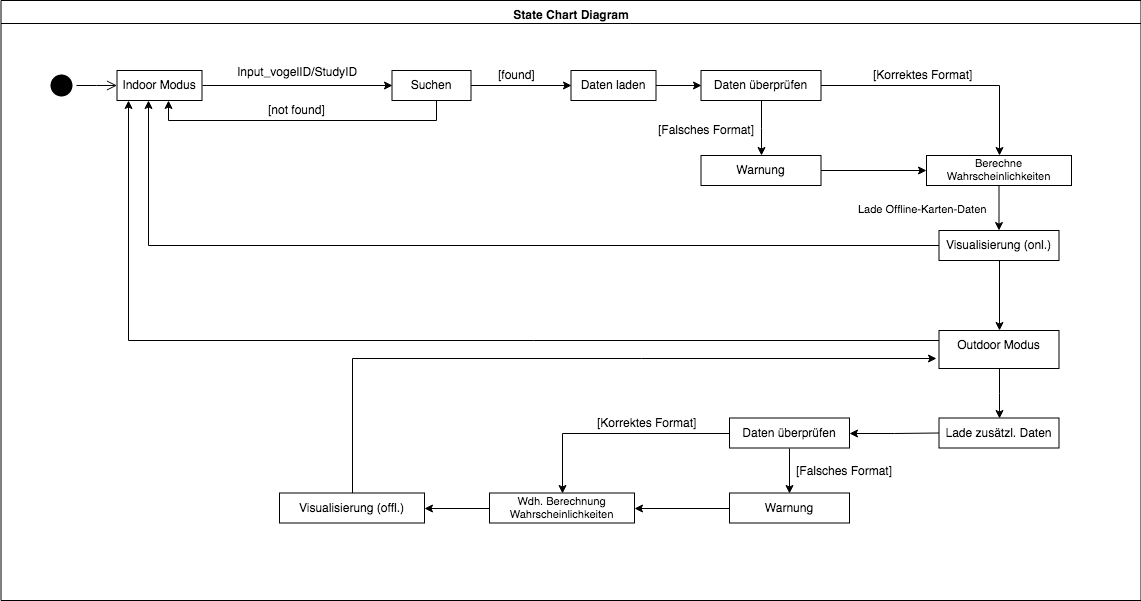
\includegraphics[width = \textwidth]{Diagramme/state_diagram.png}
Das Global-Software-Control-Diagram beschreibt das allgemeine Verhalten der App. Es besteht aus dem allgemeinem Ablauf der App im Indoor- (obere Hälfte) und Outdoormodus (untere Hälfte). \\
Zu Beginn befinden wir uns im Indoor-Modus und können nun mit der VogelID und StudyID nach einem Vogel suchen. Ist der Vogel nicht verfügbar, so haben wir keine Möglichkeit weiter zu machen und beginnen von vorne. Ist er vorhanden, so laden wir dessen Daten. Anschließend werden diese geprüft bzw. geparst. Im Fall, dass die Daten formal falsch sind (siehe SRS für die Definition von formal falsch), werden diese trotzdem zur Berechnung benutzt. Allerdings wird eine Warnung über die Qualität der Daten erscheinen. Nach dem Berechnen der Wahrscheinlichkeiten, werden die Kartendaten und weitere Daten für die Visualisierung heruntergeladen, um diese auch ohne Internetverbindung visualisieren zu können. Solange wir uns aber im Indoor-Modus befinden, können diese mit Cesium visualisiert werden. Sollen andere Vögel untersucht werden, so kann die Suche von vorne beginnen. \\
Geht der Forscher nun in das Feld, schaltet dieser in den Outdoor-Modus. Der Ablauf ist nun ähnlich wie im Indoor-Modus. Es können zusätzliche oder neue Daten des Vogels über die mobilen Daten geladen werden. Sie fließen in die erneute Wahrscheinlichkeitsberechnung ein und aktualisieren die Visualisierung, die nun allerdings mit einem Offline-Karten-Provider dargestellt wird. \\


% • How will control signals be used?
% • How do the subsystems communicate? --> interface descriptions?
% • How do the subsystems synchronize? --> statechart diagram? Concurrency


\subsubsection{Interfaces}
\label{sec:interfaces}


% ----

% Übersetzung?
\subsection{Boundary Conditions}
{\color{red}{Oliver}}
% Sequenzdiagramm?
% \includegraphics[width = 0.8\textwidth]{pictures/SeqDia.png}

% Startup behaviour (What happens, when we start the system?)
% • Shutdown behaviour (What happens, when we stop the system?)
% • Failure behaviour (What happens, when the system
% missbehaves? Which kind of failures can you imagine? What
% does the system need to do then?)



\section{Anhänge}

\subsection{Geänderte Anforderungen}

% List changed requirements in old and new form.

%----------------------------------------------------------------------------------------

\end{document}